\documentclass{article}

\usepackage[preprint]{neurips_2026}   % preprint: muestra autores y sin números de línea

\usepackage[utf8]{inputenc}
\usepackage[T1]{fontenc}
\usepackage{babel}
\babelprovide[import, main]{spanish}   % no hay spanish.ldf instalado: se usa el locale de babel
\usepackage{hyperref}
\hypersetup{hidelinks}                 % enlaces sin recuadros de color
\AtBeginDocument{\renewcommand{\tablename}{Tabla}}
\usepackage{url}
\usepackage{booktabs}
\usepackage{amsfonts}
\usepackage{amsmath}
\usepackage{nicefrac}
\usepackage{microtype}
\usepackage{xcolor}
\usepackage{graphicx}
\usepackage{multirow}


% mismo estilo que el resumen de neurips_2026.sty, con el título en español
\renewenvironment{abstract}{\vskip 0.075in\centerline{\large\bf Resumen}\vspace{0.5ex}\begin{quote}}{\par\end{quote}\vskip 1ex}

\title{Clasificación multietiqueta de anomalías de rodilla en resonancia magnética con CNN y aprendizaje débilmente supervisado}

\author{%
  Alvaro Alejandro Siesquén Abad \And Sergio Alonso Ortiz Pauca \AND
  Alfonso Pérez Ramos \And Kiara Isumi Álvarez Barrionuevo \\
  Facultad de Ingeniería Industrial y de Sistemas, Universidad Nacional de Ingeniería, Lima, Perú
}

\begin{document}

\maketitle

\begin{abstract}
Predecimos 12 hallazgos clínicos en resonancias magnéticas (RM) de rodilla del conjunto RSNA Knee Abnormality Detection, en el que solo 58 de 4407 estudios tienen etiqueta de radiólogo. Para los demás construimos etiquetas débiles a partir del informe radiológico, escrito en texto libre y en nueve idiomas. Combinamos reglas multilingües con una regresión logística sobre embeddings de EmbeddingGemma, y la etiqueta híbrida alcanza un AUC de 0,856 frente al radiólogo, con un ruido estimado de 17,8~\%. Con estas etiquetas entrenamos dos arquitecturas 2.5D que leen los tres planos de la RM: una CNN diseñada desde cero, con pirámide de características y vista con zoom, y ConvNeXt-Tiny preentrenada en ImageNet. Ambas usan pérdida focal y un esquema maestro-alumno. En los 58 estudios gold, el ensamble de 5 folds obtiene un AUC macro de 0,826 con la CNN desde cero y de \textbf{0,865} con ConvNeXt-Tiny. Las ablaciones muestran que la calidad de la etiqueta limita más que la arquitectura. Los mapas HiResCAM de ConvNeXt se concentran en las estructuras anatómicas correctas, pero revelan atajos por comorbilidad.
\end{abstract}

\section{Introducción}

La RM es la prueba de referencia para evaluar ligamentos, meniscos, cartílago y derrame en la rodilla, pero su lectura requiere radiólogos especializados y presenta variabilidad entre observadores. Un modelo que señale automáticamente los hallazgos relevantes podría servir de apoyo y priorizar estudios.

El reto RSNA Knee Abnormality Detection~\cite{rsna2026} reúne más de 5000 RM de 16 centros en cinco continentes, con informes en una docena de idiomas, y pide predecir 12 hallazgos por estudio:
\begin{itemize}
  \item roturas del ligamento cruzado anterior (LCA) y del colateral medial (LCM);
  \item roturas de menisco medial y lateral;
  \item artrosis medial, lateral y femoropatelar;
  \item derrame, sinovitis, quiste de Baker, contusión ósea y fractura.
\end{itemize}

La dificultad central es que \textbf{solo 58 estudios tienen etiqueta dorada} (\emph{gold}) de radiólogos; los 4349 restantes (\emph{silver}) solo traen el informe en texto libre. El problema es, por tanto, de aprendizaje débilmente supervisado: primero hay que construir etiquetas a partir del texto y después entrenar un clasificador de imágenes con esas etiquetas ruidosas.

Nuestras contribuciones son:
\begin{enumerate}
  \item un pipeline de etiquetas débiles multilingüe (reglas + EmbeddingGemma), validado contra gold;
  \item dos arquitecturas 2.5D multietiqueta, una CNN desde cero y otra con \emph{transfer learning}, evaluadas con validación cruzada agrupada por escáner;
  \item ablaciones de profundidad, función de pérdida, manejo del ruido de etiquetas, vista con zoom y backbone;
  \item un análisis de interpretabilidad con HiResCAM, del desbalance de clases y del sesgo geográfico y lingüístico.
\end{enumerate}

\section{Trabajos relacionados}

\paragraph{RM de rodilla con aprendizaje profundo.} MRNet~\cite{bien2018mrnet} clasificó roturas del LCA y de menisco extrayendo características de cada corte con una AlexNet preentrenada y agregándolas con \emph{max-pooling} por serie, una forma de aprendizaje con múltiples instancias. MRPyrNet~\cite{dunnhofer2021mrpyrnet} añadió una pirámide de características para no perder lesiones pequeñas al reducir la resolución, idea que adoptamos en nuestra CNN.

\paragraph{Arquitecturas CNN y \emph{transfer learning}.} ResNet~\cite{he2016resnet} introdujo los atajos residuales; DenseNet~\cite{huang2017densenet} es la base de CheXNet~\cite{rajpurkar2017chexnet}, referencia en clasificación multietiqueta de imagen médica; EfficientNet~\cite{tan2019efficientnet} escala la red de forma eficiente; y ConvNeXt~\cite{liu2022convnext} moderniza la CNN convencional con convoluciones \emph{depthwise} 7×7 y LayerNorm, sin mecanismos de atención.

\paragraph{Desbalance y etiquetas ruidosas.} La pérdida focal~\cite{lin2017focal} reduce el peso de los ejemplos fáciles, que en problemas desbalanceados son sobre todo negativos. La supervisión débil programática~\cite{ratner2017snorkel} combina fuentes ruidosas de etiquetas. Las \emph{Born-Again Networks}~\cite{furlanello2018born} re-entrenan un alumno con las predicciones de un maestro de la misma arquitectura.

\paragraph{Interpretabilidad.} Grad-CAM~\cite{selvaraju2017gradcam} pondera los mapas de una capa convolucional con el gradiente medio por canal; HiResCAM~\cite{draelos2020hirescam} usa el producto elemento a elemento de gradiente y activación, lo que lo hace fiel a la decisión del modelo en arquitecturas con \emph{pooling} no lineal.

\section{Datos y etiquetas débiles}

\paragraph{Dataset.} Cada \emph{estudio} es una RM de una rodilla con su informe. Contiene de 3 a 14 \emph{series} (5 de mediana), cada una adquirida en un plano (sagital, coronal o axial) y con una secuencia (sensible a líquido con supresión grasa, o ninguna de las dos). Cada serie tiene unos 30 \emph{cortes} 2D en DICOM, unos 819\,000 en total. Hay 83 combinaciones de fabricante, modelo, campo magnético y bobina; Siemens (44~\%), Philips (30~\%) y GE (21~\%) dominan. El 39~\% de los informes está en inglés y el resto en español, turco, croata/serbio, griego, alemán, búlgaro, neerlandés y francés.

\paragraph{Etiquetas débiles.} Partimos cada informe en cláusulas y combinamos dos fuentes:
\begin{enumerate}
  \item \textbf{Reglas multilingües}: buscan estructura + patología (por ejemplo, ``LCA'' + ``rotura'') en los 9 idiomas y clasifican la mención como de alto grado (0,9), sin grado (0,7), de bajo grado (0,35), no mencionada (0,1) o negada (0,03). Siguen los criterios oficiales: solo cuentan, por ejemplo, la rotura completa o de alto grado del LCA y el derrame moderado o grande.
  \item \textbf{Embeddings}: cada cláusula se codifica con EmbeddingGemma-300m~\cite{embeddinggemma2025}, un modelo multilingüe, y una regresión logística por hallazgo aprende a reconocer las cláusulas positivas a partir de las que las reglas etiquetaron con seguridad. Así generaliza a formulaciones e idiomas que las reglas no cubren.
\end{enumerate}
La etiqueta del estudio es la puntuación de su cláusula más fuerte. Los estudios gold nunca se usan para construir las etiquetas.

\paragraph{Combinación y validación.} Comparamos varias formas de combinar las dos fuentes contra los 58 gold (Figura~\ref{fig:comb}). La media geométrica $\sqrt{\text{reglas}\cdot\text{embeddings}}$ fue la mejor. Para comprobar que no es un ajuste al azar a esos 58 estudios, repetimos la elección dentro de gold con validación cruzada: con 4/5 de los estudios se elige la combinación y se mide en el 1/5 restante (100 particiones). La elección automática da 0,857 en datos no vistos, frente a 0,847 de la media aritmética fija. La Tabla~\ref{tab:etiquetas} resume la calidad de las etiquetas, binarizadas en 0,5 para el acuerdo y el kappa. Los embeddings ordenan bien (AUC), pero la regresión, entrenada con clases equilibradas, da probabilidades infladas: con el umbral 0,5 marca como positivo el 61~\% de los casos, de ahí su ruido alto.

\begin{figure}[t]
  \centering
  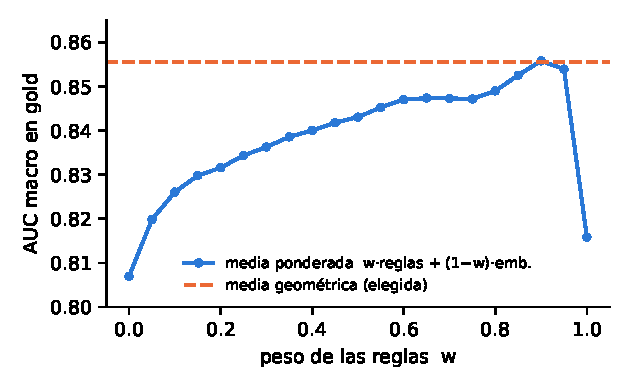
\includegraphics[width=0.48\linewidth]{figuras/combinacion_etiquetas.pdf}\hfill
  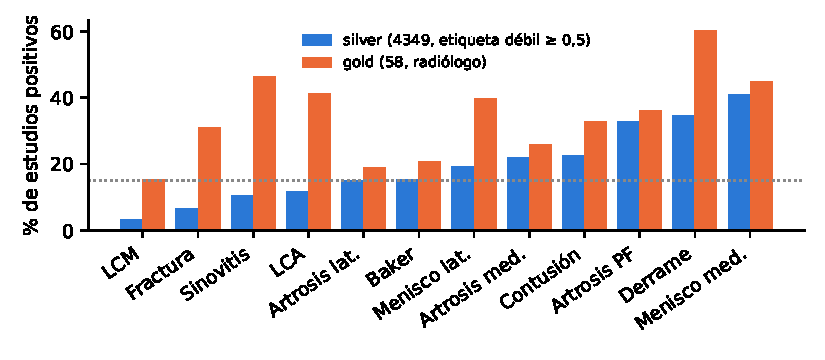
\includegraphics[width=0.5\linewidth]{figuras/prevalencia.pdf}
  \caption{\textbf{Izquierda:} AUC macro de la etiqueta débil frente a gold según la combinación de reglas y embeddings. \textbf{Derecha:} prevalencia de cada hallazgo en silver (etiqueta débil $\geq 0{,}5$) y en gold. La línea punteada marca el 15~\%, umbral que usamos para llamar \emph{raro} a un hallazgo.}
  \label{fig:comb}
\end{figure}

\begin{table}[t]
  \centering
  \caption{Calidad de las etiquetas débiles frente a los 58 estudios gold (media macro de los 12 hallazgos).}
  \label{tab:etiquetas}
  \begin{tabular}{lcccc}
    \toprule
    Fuente & AUC & Acuerdo & Ruido (1 $-$ acuerdo) & Kappa \\
    \midrule
    Reglas & 0,816 & 81,3~\% & 18,7~\% & 0,538 \\
    Embeddings$^{*}$ & 0,807 & 64,4~\% & 35,6~\% & 0,365 \\
    Híbrido, media aritmética & 0,843 & 78,9~\% & 21,1~\% & 0,521 \\
    \textbf{Híbrido, media geométrica (final)} & \textbf{0,856} & \textbf{82,2~\%} & \textbf{17,8~\%} & \textbf{0,578} \\
    \bottomrule
  \end{tabular}
\end{table}

Por hallazgo, el ruido va del 6,9~\% del LCA al 32,8~\% de la sinovitis. Los hallazgos más ruidosos son los que el informe describe de forma ambigua, como la sinovitis frente al derrame o el esguince frente a la rotura del LCM.

\paragraph{Preprocesado de imágenes.} Por estudio elegimos una serie por plano, prefiriendo la sensible a líquido con supresión grasa. Ordenamos los cortes por su posición física y aplicamos un recorte central de 150~mm según el tamaño real del píxel. Normalizamos la intensidad con los percentiles 1--99,5 y guardamos cada serie a 320×320~px.

El lado de la rodilla se toma del DICOM o del informe (69~\% de los estudios); para el resto lo completa una CNN pequeña, que acierta un 98,6~\% en validación cruzada. Las rodillas izquierdas se reflejan para que el compartimento medial quede siempre en el mismo lado de la imagen.

\paragraph{Validación.} Los 4349 estudios silver se reparten en 5 folds con \texttt{GroupKFold} agrupando por escáner, de modo que el modelo se valida siempre en escáneres que no vio, como ocurrirá con el test de otros centros. Gold queda fuera y solo se usa para la evaluación final.

\section{Metodología}

\paragraph{Entrada 2.5D y agregación por estudio.} De cada plano tomamos 12 cortes repartidos a lo largo de la serie. Cada corte se apila con sus dos vecinos como los 3 canales de una imagen, así que cada estudio aporta 36 imágenes. Cada imagen se ve dos veces:
\begin{itemize}
  \item la \textbf{vista completa}, de 150~mm a 224~px;
  \item una \textbf{vista con zoom}, los 100~mm centrales a 224~px.
\end{itemize}
La misma CNN convierte cada imagen en un vector; los vectores de las dos vistas se concatenan y la cabeza resume las 36 ventanas con media y máximo antes de una capa lineal con 12 salidas sigmoides independientes. Es un esquema de aprendizaje con múltiples instancias: la etiqueta es del estudio, no del corte.

\paragraph{Arquitectura 1: CNN desde cero (1,25~M parámetros).} El \emph{stem} tiene tres convoluciones 3×3 y \emph{max-pooling}; le siguen cuatro etapas de dos convoluciones 3×3 con BatchNorm y ReLU, de 32 a 256 canales. Una \textbf{pirámide de características}~\cite{dunnhofer2021mrpyrnet}, en la línea de las hipercolumnas y las FPN~\cite{hariharan2015hypercolumns,lin2017fpn}, junta el \emph{pooling} global (media y máximo, con LayerNorm) de las etapas 2, 3 y 4, para no perder lesiones pequeñas al reducir la resolución.

\paragraph{Arquitectura 2: ConvNeXt-Tiny preentrenada (27,9~M parámetros).} Usamos el extractor de características de ConvNeXt-Tiny~\cite{liu2022convnext}, con pesos de ImageNet, normalización de ImageNet y la misma cabeza que la arquitectura 1. Elegimos ConvNeXt entre cuatro backbones (Sección~\ref{sec:ablaciones}).

\paragraph{Entrenamiento.}
\begin{itemize}
  \item \textbf{Pérdida focal}~\cite{lin2017focal} con $\gamma = 2$ y etiquetas blandas.
  \item \textbf{Optimizador:} AdamW con \emph{weight decay} $10^{-4}$ y política OneCycle; se guarda la última época.
  \item \textbf{Arquitectura 1:} 30 épocas, lr $10^{-3}$, lote de 8 estudios.
  \item \textbf{Arquitectura 2:} 15 épocas; lr $10^{-4}$ para el backbone y $10^{-3}$ para la cabeza; lote de 2 estudios con acumulación de gradiente ×4.
  \item \textbf{Predicción final:} promedio de las probabilidades de los modelos de los 5 folds.
\end{itemize}

\paragraph{Maestro-alumno.} Un primer modelo (\emph{maestro}, arquitectura 1) se entrena en 5 folds con las etiquetas débiles. Su predicción fuera de fold para cada estudio silver se lleva, percentil a percentil, a la escala de la etiqueta débil y se mezcla con ella:
$$y_{\text{nueva}} = 0{,}5\, y_{\text{débil}} + 0{,}5\, \hat{y}_{\text{maestro}}.$$
Las dos arquitecturas finales (\emph{alumnos}) se entrenan con $y_{\text{nueva}}$. Como cada maestro vio los estudios de validación de los demás folds, la validación interna de los alumnos queda inflada, en unos +0,02 de AUC según un experimento con maestros que no ven el fold de validación. Por eso las comparaciones finales usan solo gold, que ningún paso del entrenamiento tocó.

\section{Experimentos y resultados}

\subsection{Ablaciones}
\label{sec:ablaciones}

Las ablaciones se hicieron sobre la arquitectura 1, cambiando un solo factor cada vez. Salvo la última, se hicieron con la versión anterior de las etiquetas (media aritmética), así que lo comparable son las diferencias entre variantes. La variación entre folds es de 0,01--0,02 de AUC, por lo que las conclusiones clave se confirmaron con validación cruzada de 5 folds (Tabla~\ref{tab:ablacion}).

\begin{table}[t]
  \centering
  \caption{Ablaciones sobre la arquitectura 1. AUC macro en validación (etiquetas débiles) y en gold. ``5f'': media de 5 folds; ``ens.'': ensamble de los 5 modelos; el resto, fold 0.}
  \label{tab:ablacion}
  \small
  \begin{tabular}{llcc}
    \toprule
    Factor & Variante & AUC val & AUC gold \\
    \midrule
    \multirow{4}{*}{Profundidad} & 1 bloque por etapa, sin atajos & 0,768 & 0,746 \\
     & 2 bloques por etapa, sin atajos & 0,772 & 0,739 \\
     & 1 bloque, con atajos residuales & 0,756 & 0,738 \\
     & 2 bloques, con atajos residuales & 0,755 & 0,739 \\
    \midrule
    \multirow{2}{*}{Pérdida (5f / ens.)} & BCE & 0,776 ± 0,021 & 0,764 / 0,784 \\
     & \textbf{focal $\gamma=2$} & \textbf{0,778 ± 0,007} & \textbf{0,775 / 0,794} \\
    \midrule
    \multirow{5}{*}{Etiquetas ruidosas} & A: blandas (base) & 0,786 & 0,768 \\
     & B: binarizadas en 0,5 & 0,777 & 0,769 \\
     & C: solo alta confianza ($|y-0{,}5|>0{,}2$) & 0,780 & 0,777 \\
     & D: ponderadas por confianza $|2y-1|$ & 0,788 & 0,775 \\
     & E: híbrido calibrado & 0,770 & 0,771 \\
    \midrule
    \multirow{2}{*}{Vista (5f / ens.)} & solo vista completa & 0,778 & 0,775 / 0,794 \\
     & \textbf{completa + zoom 100~mm} & \textbf{0,785} & \textbf{0,786 / 0,797} \\
    \midrule
    \multirow{2}{*}{Etiquetas (5f / ens.)} & débiles & 0,785 & 0,786 / 0,797 \\
     & \textbf{maestro-alumno} & (inflada) & \textbf{0,808 / 0,812} \\
    \midrule
    \multirow{4}{*}{Combinación (5f)} & maestro · media aritmética & --- & 0,786 \\
     & \textbf{maestro · media geométrica} & --- & \textbf{0,790} \\
     & alumno · media aritmética & --- & 0,808 \\
     & \textbf{alumno · media geométrica} & --- & \textbf{0,822} \\
    \bottomrule
  \end{tabular}
\end{table}

\paragraph{Profundidad.} Duplicar la profundidad o añadir atajos residuales no mejora: con ~3500 estudios y etiquetas ruidosas, el problema no es optimizar una red más profunda sino generalizar.

\paragraph{Pérdida.} La pérdida focal empata en validación, pero mejora gold en 4 de 5 folds (+0,011) y reduce a un tercio la variación entre folds. No aprende mejor a imitar las etiquetas débiles, pero generaliza mejor a las del radiólogo.

\paragraph{Etiquetas ruidosas.} Binarizar las etiquetas empeora la validación ($-$0,009, IC95 [$-$0,017; $-$0,001]), porque se pierde la información de ``dudoso''. Filtrar o ponderar por confianza mejora gold en +0,007 a +0,009, pero dentro del ruido de 58 estudios.

\paragraph{Combinación de las fuentes.} Repetimos el maestro y los dos alumnos con la etiqueta de media geométrica (5 folds, misma receta). La validación interna no es comparable, porque cada versión se valida contra su propia etiqueta, así que solo comparamos en gold. Una etiqueta más fiel al radiólogo (+0,013 de AUC) da modelos algo mejores en todas las etapas: el maestro sube de 0,786 a 0,790, el alumno CNN de 0,808 a 0,822 (ensamble: de 0,812 a 0,826) y ConvNeXt de 0,842 a 0,856 de media por fold (ensamble: de 0,849 a 0,865). La mejora es pequeña, del orden de la variación entre folds, pero aparece en 4 de los 5 folds y el quinto empata.

\paragraph{Vista y plano.} El zoom mejora en 4 de 5 folds. Anular cada vista en inferencia muestra un reparto aprendido sin supervisión:
\begin{itemize}
  \item sin el zoom se hunden menisco medial ($-$0,39), LCM ($-$0,31) y LCA ($-$0,15);
  \item sin la vista completa caen derrame ($-$0,10), artrosis y Baker.
\end{itemize}
Añadir las series sin supresión grasa como entrada extra empeoró gold en $-$0,017.

\paragraph{Descartados.} Probamos y descartamos, por no mejorar de forma consistente entre folds:
\begin{itemize}
  \item compuertas \emph{squeeze-and-excitation}: +0,002 / $-$0,003;
  \item convoluciones 1D entre cortes: $-$0,008 / $-$0,013;
  \item \emph{pooling} atento por hallazgo: $-$0,015 / $-$0,033, que aprendió atajos fuera de la articulación;
  \item aumentación geométrica y EMA de los pesos: $\pm$0,003;
  \item vista completa a 320~px: $-$0,002;
  \item una CNN multiescala tipo Inception como alternativa de diseño propio: $-$0,010 / +0,012.
\end{itemize}

\paragraph{Backbone preentrenado.} En el fold 0, ResNet-50, EfficientNet-B0 y DenseNet-121 obtuvieron 0,822--0,825 en gold, y ConvNeXt-Tiny 0,836. Fue el único con el IC95 de la mejora sobre nuestra CNN por encima de cero: +0,034 [+0,013; +0,056].

\subsection{Resultados finales}

\begin{table}[t]
  \centering
  \caption{Modelos finales (ensamble de 5 folds). AUC macro en los 58 gold con IC95 por \emph{bootstrap} (2000 remuestreos), AUC fuera de fold (OOF) en los 4349 silver frente a la etiqueta débil, precisión, recall y F1 con el umbral de Youden elegido en OOF.}
  \label{tab:final}
  \footnotesize
  \setlength{\tabcolsep}{4pt}
  \begin{tabular}{lccccc}
    \toprule
    Modelo & AUC gold [IC95] & AUC OOF & Precisión & Recall & F1 \\
    \midrule
    Arq. 1 · CNN desde cero & 0,826 [0,779--0,868] & 0,822 & 0,543 & 0,847 & 0,645 \\
    Arq. 2 · ConvNeXt-Tiny & \textbf{0,865 [0,827--0,898]} & \textbf{0,839} & \textbf{0,549} & \textbf{0,887} & \textbf{0,665} \\
    \bottomrule
  \end{tabular}
\end{table}

ConvNeXt supera a la CNN desde cero en los 5 folds: +0,039 [+0,017; +0,064] en el ensamble. Gana sobre todo en estructuras finas: menisco lateral, LCA, fractura y menisco medial, entre +0,05 y +0,10 (Figura~\ref{fig:auc}). Promediar las dos arquitecturas empeora (0,854). Con ConvNeXt, los mejores hallazgos son la artrosis medial, el derrame y el menisco medial ($\geq$0,95); los peores, el LCM (0,76) y la sinovitis (0,71).

\begin{figure}[t]
  \centering
  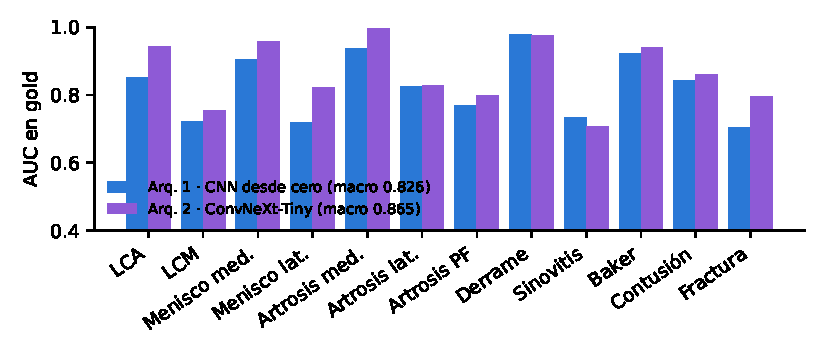
\includegraphics[width=0.75\linewidth]{figuras/auc_por_hallazgo.pdf}
  \caption{AUC por hallazgo en gold de los ensambles de 5 folds de las dos arquitecturas.}
  \label{fig:auc}
\end{figure}

\paragraph{Umbral.} Para convertir probabilidades en sí/no usamos un umbral por hallazgo y por modelo, elegido en OOF con el índice de Youden (máximo de sensibilidad + especificidad $-$ 1) y aplicado sin cambios a gold.

La razón es que gold está enriquecido respecto a silver: fractura ×4,7, sinovitis ×4,3, LCA ×3,5 (Figura~\ref{fig:comb}). Youden no depende de la prevalencia, a diferencia del máximo F1. Prioriza el recall (0,887), adecuado para un sistema de apoyo que no debe perder lesiones. Un umbral fijo de 0,5 da un F1 macro parecido (0,680), pero hunde el recall de los hallazgos raros (0,38).

\section{Interpretabilidad}

Calculamos mapas HiResCAM~\cite{draelos2020hirescam} a la salida de la tercera etapa de cada red (14×14). Como la red decide con las 72 imágenes del estudio, el mapa se calcula a la vez para todas, con el gradiente del logit del estudio. Así se obtiene qué cortes usó la red y qué zona de cada corte. Preferimos HiResCAM a Grad-CAM porque el \emph{max-pooling} espacial concentra el gradiente: el promedio por canal de Grad-CAM producía mapas difusos y, en ocasiones, fuera de la rodilla.

La Figura~\ref{fig:gradcam} muestra dos hallazgos; el repositorio incluye también menisco medial y derrame. Con ConvNeXt, el mapa del LCA se concentra en la escotadura intercondílea de un corte sagital central, justo sobre el ligamento, con el 20~\% del mapa en una sola ventana. El del quiste de Baker cae sobre la colección líquida posterior en cortes coronales, sagitales y axiales. En el derrame, el mapa se sitúa en el receso suprarrotuliano de los cortes sagitales, donde se acumula el líquido.

La Tabla~\ref{tab:planos} resume, sobre todos los positivos gold, qué planos usa cada red. Comparar con un único plano «esperado» resulta engañoso: el derrame y el quiste de Baker se ven en los tres planos, y ConvNeXt los localiza sobre todo en cortes coronales. En el menisco medial, ConvNeXt concentra el 58~\% del mapa en el plano coronal, el natural para esa estructura. Nuestra CNN reparte más el mapa entre planos y ventanas, salvo en el quiste de Baker, que mira sobre todo en axial (53~\%).

\begin{figure}[t]
  \centering
  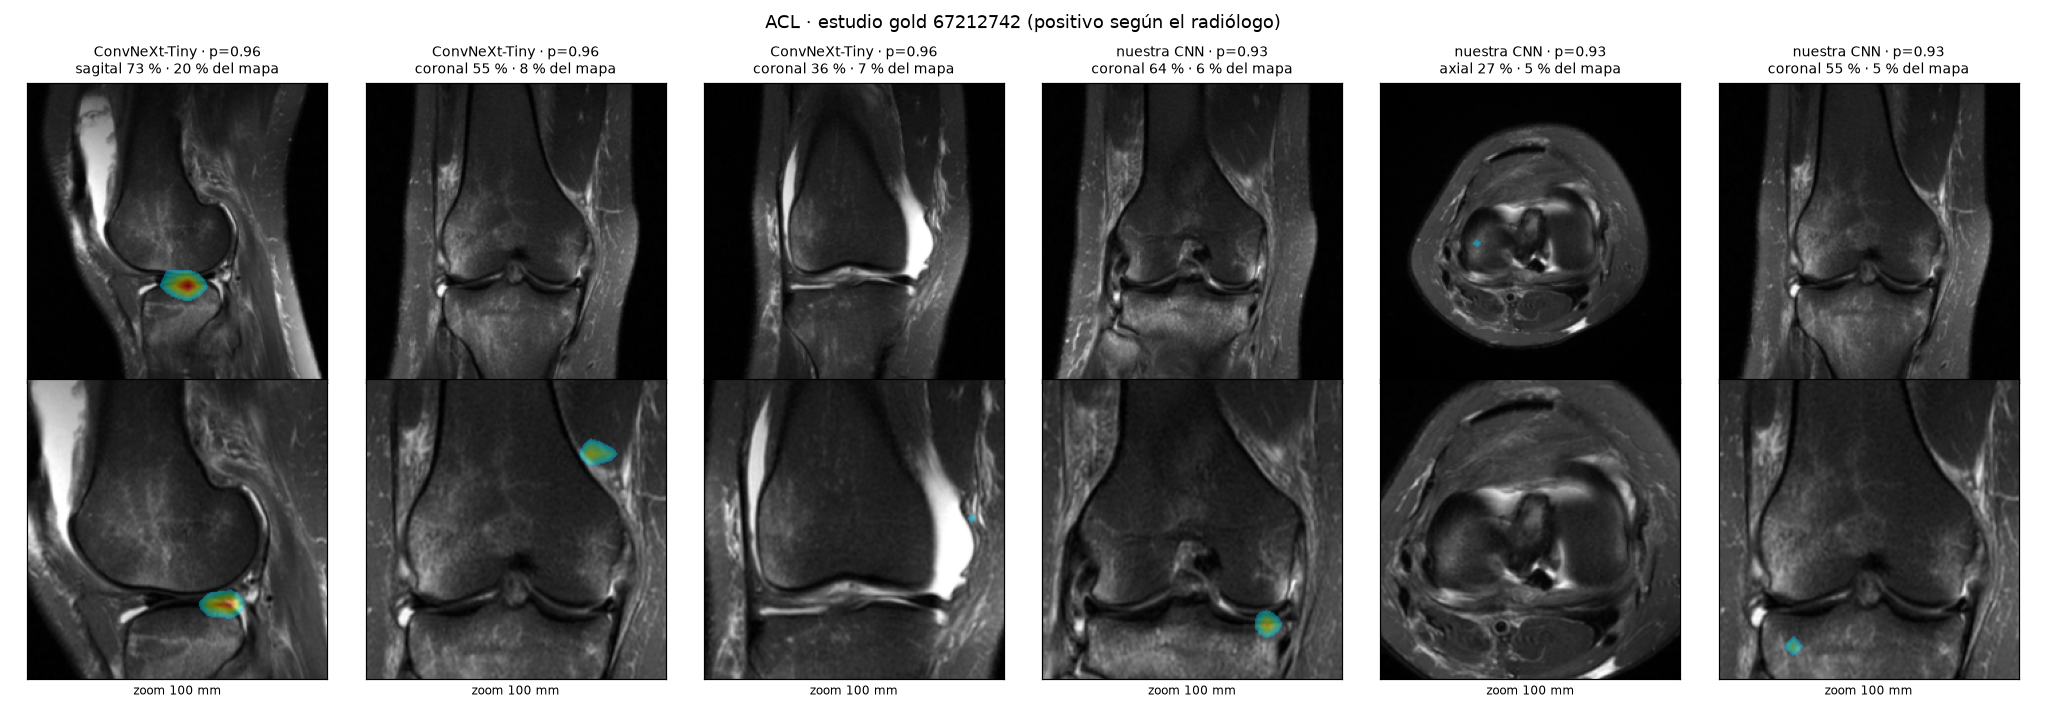
\includegraphics[width=\linewidth]{figuras/gradcam_acl.png}\\[2pt]
  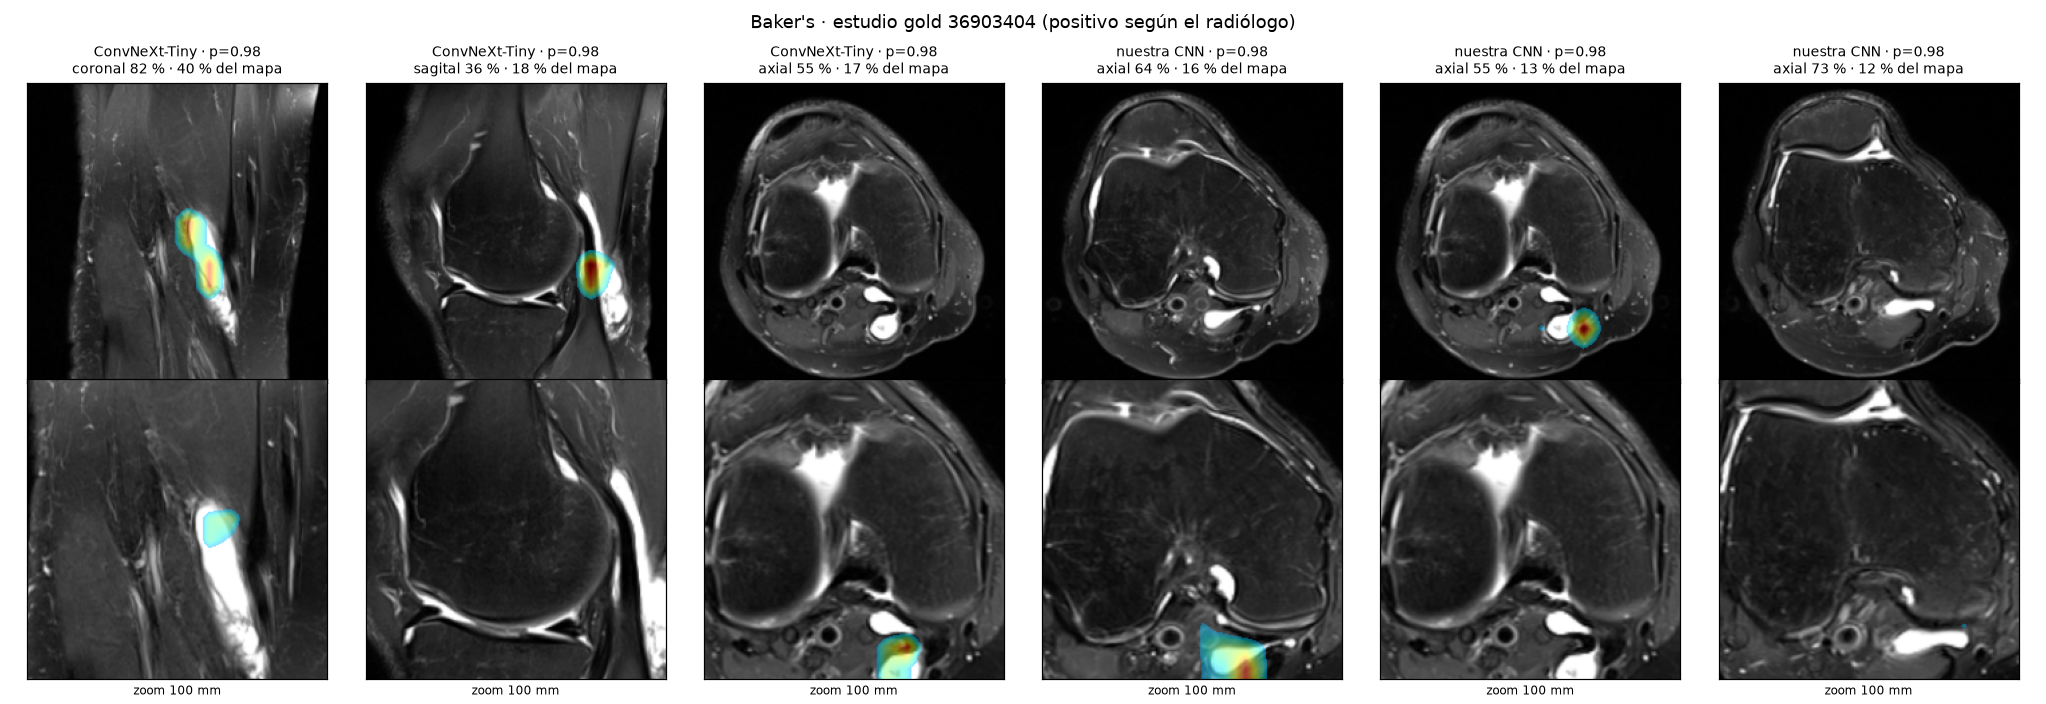
\includegraphics[width=\linewidth]{figuras/gradcam_baker.png}
  \caption{HiResCAM en un estudio gold positivo para LCA (arriba) y quiste de Baker (abajo). Por modelo, las 3 ventanas con más peso del mapa: vista completa (fila superior) y zoom (inferior). Izquierda: ConvNeXt-Tiny; derecha: CNN desde cero.}
  \label{fig:gradcam}
\end{figure}

\begin{table}[t]
  \centering
  \caption{Porcentaje del mapa HiResCAM en cada plano, promediado sobre los positivos gold de cada hallazgo (33~\% = sin preferencia). Modelos del fold 0.}
  \label{tab:planos}
  \small
  \begin{tabular}{lcccccc}
    \toprule
    & \multicolumn{3}{c}{ConvNeXt-Tiny} & \multicolumn{3}{c}{CNN desde cero} \\
    \cmidrule(lr){2-4}\cmidrule(lr){5-7}
    Hallazgo (positivos) & sag. & cor. & ax. & sag. & cor. & ax. \\
    \midrule
    LCA (24) & 38 & \textbf{43} & 19 & 27 & \textbf{40} & 33 \\
    Menisco medial (26) & 24 & \textbf{58} & 18 & 28 & \textbf{42} & 30 \\
    Derrame (35) & 36 & \textbf{44} & 20 & 33 & 35 & 32 \\
    Baker (12) & 25 & \textbf{53} & 22 & 20 & 28 & \textbf{53} \\
    \bottomrule
  \end{tabular}
\end{table}

Los mapas también revelan un \textbf{atajo por comorbilidad}. En el estudio con rotura de menisco medial, las ventanas principales de ConvNeXt están sobre la escotadura intercondílea, donde están los ligamentos cruzados, y no sobre el menisco; las roturas de menisco medial suelen acompañar a las del LCA. Nuestra CNN, en cambio, marca los bordes de los meniscos en la vista con zoom. La correlación es real, pero es una pista indirecta: con etiquetas a nivel de estudio, la red no sabe dónde está cada lesión y usa todo lo que correlaciona.

\section{Desbalance de clases}

Con las etiquetas finales, cuatro hallazgos tienen menos del 15~\% de positivos en silver: LCM (3,4~\%), fractura (6,6~\%), sinovitis (10,7~\%) y LCA (11,8~\%). Los más frecuentes son menisco medial (41~\%), derrame (35~\%) y artrosis femoropatelar (33~\%), como muestra la Figura~\ref{fig:comb}.

Los raros rinden peor en gold que los frecuentes: 0,800 frente a 0,898 con ConvNeXt. Sin embargo, frente a la etiqueta débil (OOF) rinden igual o mejor: 0,851 frente a 0,833. Es decir, la red imita bien la etiqueta débil, pero esta es peor en los raros, que el informe menciona menos y de forma más ambigua.

Evaluamos tres estrategias de mitigación:
\begin{enumerate}
  \item \textbf{Pérdida focal}, que concentra el gradiente en los ejemplos difíciles. En el experimento controlado BCE frente a focal:
  \begin{itemize}
    \item raros: +0,007 en validación y +0,028 en gold;
    \item frecuentes: $-$0,012 y +0,010.
  \end{itemize}
  \item \textbf{Umbral por hallazgo}: en los raros, el recall sube de 0,38 a 0,88 y el F1 de 0,48 a 0,60, sin reentrenar.
  \item \textbf{Vista con zoom y ensamble}: ayudan sobre todo a las lesiones pequeñas; fractura y LCA mejoran +0,07 y +0,06 con ConvNeXt.
\end{enumerate}
El análisis indica que el siguiente paso más prometedor es mejorar la etiqueta de los raros, más que reponderar la pérdida.

\section{Sesgo geográfico y lingüístico}

Los datos provienen de 16 centros en cinco continentes, con informes en varios idiomas, y el sesgo puede entrar por dos vías.

\paragraph{Lingüística.} Las etiquetas débiles salen del texto. Las reglas cubren 9 idiomas, pero las escribimos nosotros, con más soltura en español e inglés, y los organizadores mencionan 12 idiomas, así que el test puede contener idiomas ausentes en entrenamiento. Además, cada escuela radiológica usa umbrales y vocabulario distintos. Por ejemplo, un ``leve derrame'' en turco no cumple el criterio de derrame moderado.

Medido frente a la etiqueta débil, el AUC fuera de fold de ConvNeXt varía con el idioma del informe: de 0,864 en español y 0,854 en inglés a 0,798 en croata/serbio y 0,808 en griego (Figura~\ref{fig:sesgo}). Esta diferencia mezcla calidad del modelo y calidad de la etiqueta en cada idioma. Precisamente por eso indica que los idiomas menos cubiertos reciben una supervisión de peor calidad.

\paragraph{Geográfica y técnica.} Cada centro tiene escáneres, protocolos y poblaciones propios. El AUC varía también por fabricante, de 0,820 en Siemens a 0,858 en GE, y entre folds (0,825--0,856), que agrupan escáneres distintos. Mitigamos este efecto de tres formas:
\begin{itemize}
  \item validamos siempre en escáneres no vistos;
  \item normalizamos la escala física (recorte de 150~mm) y la intensidad (percentiles);
  \item usamos un modelo de embeddings multilingüe, que transfiere lo aprendido entre idiomas.
\end{itemize}

Aun así, los 58 gold no permiten medir el rendimiento por centro o por idioma con fiabilidad, y una población poco representada, por ejemplo de Sudamérica, podría recibir un modelo peor calibrado. Antes de un uso clínico haría falta una validación externa por región e idioma.

\begin{figure}[t]
  \centering
  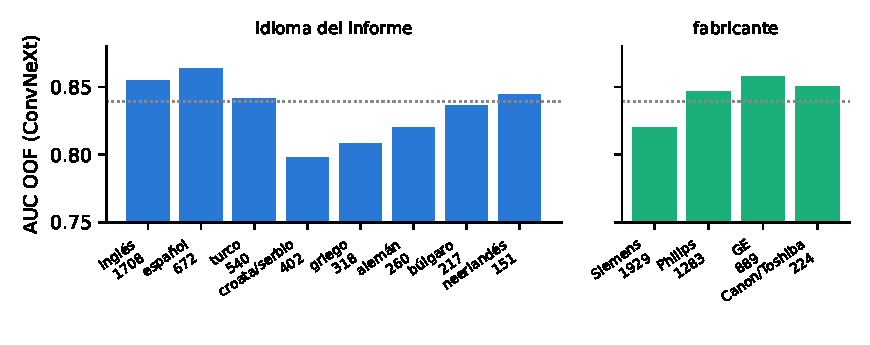
\includegraphics[width=0.7\linewidth]{figuras/sesgo.pdf}
  \caption{AUC fuera de fold de ConvNeXt-Tiny (frente a la etiqueta débil) por idioma del informe y por fabricante del escáner. Bajo cada barra, el número de estudios; la línea punteada es el AUC global.}
  \label{fig:sesgo}
\end{figure}

\section{Limitaciones y conclusiones}

\paragraph{Limitaciones.}
\begin{itemize}
  \item \textbf{Gold pequeño.} Con 58 estudios, los intervalos de confianza son anchos (±0,04 en el AUC macro) y el LCM tiene solo 9 positivos.
  \item \textbf{Reutilización de gold.} La combinación de etiquetas se eligió con gold, que también es el conjunto de evaluación. La validación cruzada dentro de gold mitiga, pero no elimina, ese sesgo.
  \item \textbf{Validación interna inflada.} La validación de los alumnos del maestro-alumno está inflada por la filtración descrita.
  \item \textbf{Resolución de los mapas.} HiResCAM a 14×14 localiza regiones, no estructuras.
  \item \textbf{Sin validación clínica.} Ningún resultado se validó en un contexto clínico real.
\end{itemize}

\paragraph{Conclusiones.} Con solo 58 estudios etiquetados por expertos, un pipeline de etiquetas débiles multilingüe permite entrenar clasificadores de RM de rodilla competitivos: 0,865 de AUC en gold. Las lecciones principales son tres:
\begin{itemize}
  \item el \emph{transfer learning} desde ImageNet aporta más (+0,039) que cualquier cambio de arquitectura de diseño propio;
  \item la calidad de la etiqueta, mejorada con el híbrido y el maestro-alumno, es el factor limitante, sobre todo en los hallazgos raros;
  \item la interpretabilidad confirma una atención anatómicamente plausible, pero también atajos que conviene vigilar.
\end{itemize}
El código es reproducible de extremo a extremo con un solo comando: \url{https://github.com/sergio100899/rsna-knee-multilabel-cnn}.

\bibliographystyle{plainnat}
\bibliography{referencias}

\end{document}
